\section{Cutting Tool and Cutting Tool Archetype} 
\label{cutting-tool-and-cutting-tool-archetype}
There are two \glspl{information model} used to represent a cutting tool, \gls{cuttingtoolarchetype} and \gls{cuttingtool}.  The \gls{cuttingtoolarchetype} represent the static cutting tool geometries and nominal values as one would expect from a tool catalog and the \gls{cuttingtool} represents the use or application of the tool on the shop floor with actual measured values and process data.  In Version 1.3.0 of the MTConnect Standard it was decided to separate out these two concerns since not all pieces of equipment will have access to both sets of information.  In this way, a generic definition of the cutting tool can coexist with a specific assembly \gls{information model} with minimal redundancy of data.

\subsection{XML Schema Structure for CuttingTool and CuttingToolArchetype}
The \fig{cuttingtool-schema} shows the XML schema that applies to both the \gls{cuttingtool} \gls{information model} and the \gls{cuttingtoolarchetype} \gls{information model}.

\begin{figure}[ht]
  \centering
  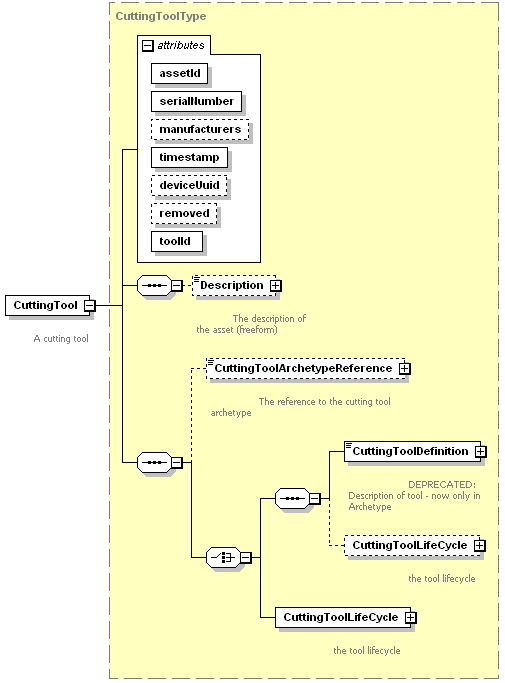
\includegraphics[width=0.75\textwidth]{figures/cuttingtool-schema.png}
  \caption{Cutting Tool Schema}
  \label{fig:cuttingtool-schema}
\end{figure}

\FloatBarrier

\begin{note}
Note: The use of the XML element \gls{cuttingtooldefinition} has been \DEPRECATED in the \gls{cuttingtool} schema, but remains in the \gls{cuttingtoolarchetype} schema.

\end{note}

The following sections contain the definitions of \gls{cuttingtool} and \gls{cuttingtoolarchetype} and describe their unique components. The following are the common entities for both elements.

\subsection{Common Attributes for CuttingTool and CuttingToolArchetype}
\label{sec:Common Attributes for CuttingTool and CuttingToolArchetype}

\tabulinesep = 5pt
\begin{longtabu} to \textwidth {
    |l|X[3l]|X[0.75l]|}
\caption{Attributes for CuttingTool and CuttingToolArchetype} \label{table:attributes-for-cuttingtool-and-cuttingtoolarchetype} \\

\hline
Attribute & Description & Occurrence \\
\hline
\endfirsthead

\hline
\multicolumn{3}{|c|}{Continuation of Table \ref{table:attributes-for-cuttingtool-and-cuttingtoolarchetype}}\\
\hline
Attribute & Description & Occurrence \\
\hline
\endhead

\gls{timestamp}
&
The time this \gls{mtconnect asset} was last modified. Always given in UTC. The \gls{timestamp} \MUST be provided in UTC (Universal Time Coordinate, also known as GMT). This is the time the \gls{asset} data was last modified.
\newline \gls{timestamp} is a required attribute.
&
1 \\
\hline
 
\gls{assetid}
&
The unique identifier of the instance of this tool. This will be the
same as the \gls{toolid} and \gls{serialnumber} in most cases. The \gls{assetid} \SHOULD be the combination of the \gls{toolid} and \gls{serialnumber} as in \gls{toolid}. \gls{serialnumber} or an equivalent implementation dependent identification scheme.
\newline \gls{assetid} is a required attribute.
\newline \gls{assetid} is a permanent identifier that will be associated with an \gls{mtconnect asset} for its entire life.
&
1 \\
\hline

\gls{serialnumber}
&
The unique identifier for this assembly. This is defined as an XML string type and is implementation dependent.
\newline \gls{serialnumber} is a required attribute.
&
1 \\
\hline

\gls{toolid}
&
The identifier for a class of Cutting Tools. This is defined as an XML string type and is implementation dependent.
\newline \gls{toolid} is a required attribute.
&
1 \\
\hline

\gls{deviceuuid}
&
\glsentrydesc{deviceuuid}
&
1 \\
\hline

\gls{manufacturers}
&
An optional attribute referring to the manufacturer(s) of this Cutting
Tool, for this element, this will reference the Tool Item and Adaptive
Items specifically. The Cutting Items manufacturers’ will be an
attribute of the \gls{cuttingitem} elements. The representation will be a
comma (,) delimited list of manufacturer names. This can be any
series of numbers and letters as defined by the XML type \cfont{string}.
&
0..1 \\
\hline

\gls{removed}
&
This is an indicator that the Cutting Tool has been removed from the piece of equipment.
\newline \gls{removed} is a required attribute.
\newline If the \gls{mtconnect asset} is marked as removed, it will not be visible to the client application unless the \cfont{includeRemoved=true} parameter is provided in the URL. If this attribute is not present it \MUST be assumed to be \cfont{false}. The value is an \cfont{xsi:boolean} type and \MUST be \cfont{true} or \cfont{false}.
&
0..1 \\
\hline


\end{longtabu}

\pagebreak

\subsection{Common Elements for CuttingTool and CuttingToolArchetype}


\tabulinesep = 5pt
\begin{longtabu} to \textwidth {
    |l|X[3l]|X[0.75l]|}
\caption{Common Elements for CuttingTool and CuttingToolArchetype} \label{table:elements-for-cuttingtool-and-cuttingtoolarchetype} \\

\hline
Element & Description & Occurrence \\
\hline
\endfirsthead

\hline
\multicolumn{3}{|c|}{Continuation of Table \ref{table:elements-for-cuttingtool-and-cuttingtoolarchetype}}\\
\hline
Element & Description & Occurrence \\
\hline
\endhead

\gls{description}	
&
An element that can contain any descriptive content. This can contain configuration information and manufacturer specific details. This element is defined to contain mixed content and XML elements can be added to extend the descriptive semantics of MTConnect Standard.
&
0..1 \\
\hline


\end{longtabu}



\subsubsection{Description Element for CuttingTool and CuttingToolArchetype}
\gls{description} \MAY contain mixed content, meaning that an additional XML element or plain text may be provided as part of the content of the description tag.  Currently \gls{description} contains no attributes.

\section{CuttingToolArchetype Information Model}
The \gls{cuttingtoolarchetype} \gls{information model} will have the identical structure as the \gls{cuttingtool} \gls{information model} illustrated in \fig{cuttingtool-schema}, except for a few entities.  The \gls{cuttingtool} will no longer carry the \gls{cuttingtooldefinition}, this \MUST only appear in the \gls{cuttingtoolarchetype}.  The \gls{cuttingtoolarchetype} \MUSTNOT have measured values and \MUSTNOT have any of the following items: \gls{cutterstatus}, \gls{toollife} values, \gls{location}, or a \gls{reconditioncount}. 

MTConnect Standard will adopt the ISO 13399 structure when formulating the vocabulary for Cutting Tool geometries and structure to be represented in the \gls{cuttingtoolarchetype}.  The nominal values provided in the \gls{cuttingtoollifecycle} section are only concerned with two aspects of the Cutting Tool, the Cutting Tool and the Cutting Item.  The Tool Item, Adaptive Item, and Assembly Item will only be covered in the \gls{cuttingtooldefinition} section of this document since this section contains the full ISO 13399 information about a Cutting Tool.

\begin{figure}[ht]
  \centering
  \scalebox{0.7}{
  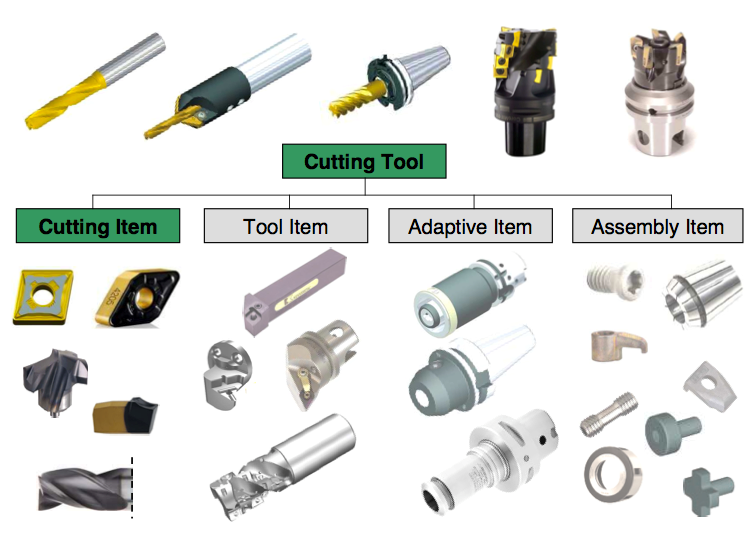
\includegraphics[width=1.0\textwidth]{figures/cutting-tool-parts.png}
  }
  \caption{Cutting Tool Parts}
  \label{fig:cutting-tool-parts}
\end{figure}

\FloatBarrier

The \fig{cutting-tool-parts} illustrates the parts of a Cutting Tool.  The Cutting Tool is the aggregate of all the components and the Cutting Item is the part of the tool that removes the material from the workpiece.  These are the primary focus of the MTConnect Standard. 

\begin{figure}[ht]
  \centering
  \scalebox{0.7}{
  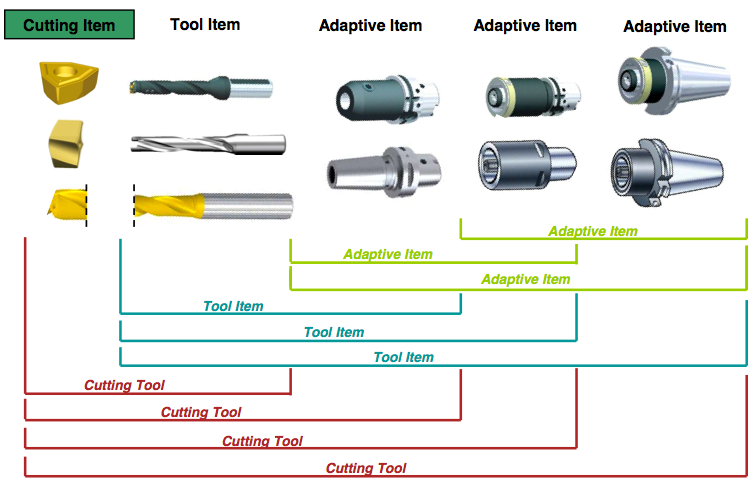
\includegraphics[width=1.0\textwidth]{figures/cutting-tool-composition.png}
  }
  \caption{Cutting Tool Composition}
  \label{fig:cutting-tool-composition}
\end{figure}

\FloatBarrier

\fig{cutting-tool-composition} provides another view of the composition of a Cutting Tool.  The Adaptive Items and Tool Items will be used for measurements, but will not be modeled as separate entities.  When we are referencing the Cutting Tool we are referring to the entirety of the assembly and when we provide data regarding the Cutting Item we are referencing each individual item as illustrated on the left of the previous diagram.

\fig{cutting-tool-tool-item-cutting-item} and \fig{cutting-tool-tool-item-cutting-item-2} further illustrates the components of the Cutting Tool.  As we compose the Tool Item, Cutting Item, Adaptive Item, we get a Cutting Tool.  The Tool Item, Adaptive Item, and Assembly Item will only be in the \gls{cuttingtooldefinition} section that will contain the full ISO 13399 information.

\begin{figure}[ht]
  \centering
  \scalebox{0.7}{
  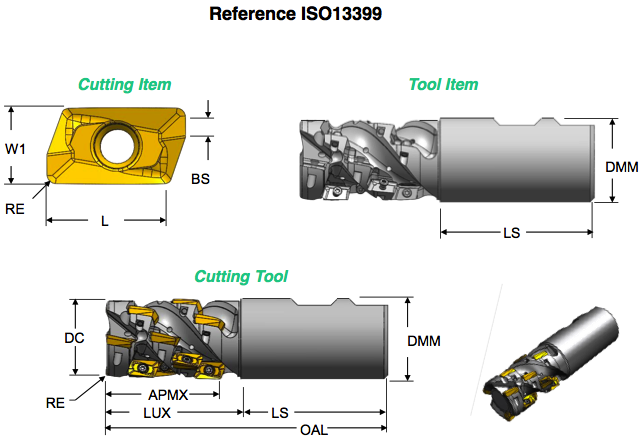
\includegraphics[width=1.0\textwidth]{figures/cutting-tool-tool-item-cutting-item.png}
  }
  \caption{Cutting Tool, Tool Item, and Cutting Item}
  \label{fig:cutting-tool-tool-item-cutting-item}
\end{figure}

\FloatBarrier

\begin{figure}[ht]
  \centering
  \scalebox{0.7}{
  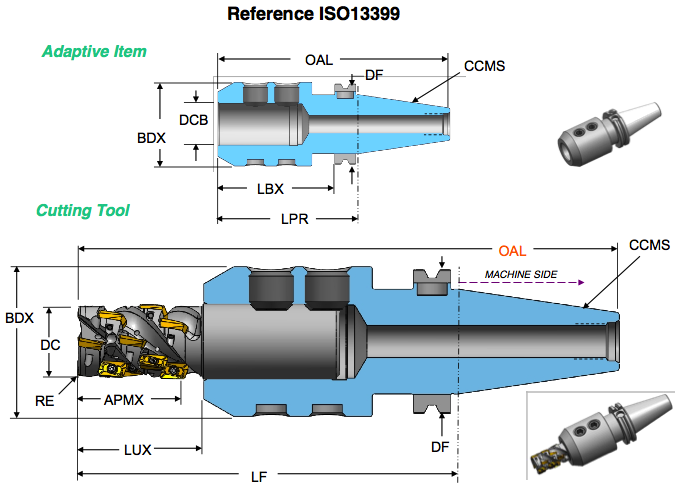
\includegraphics[width=1.0\textwidth]{figures/cutting-tool-tool-item-cutting-item2.png}
  }
  \caption{Cutting Tool, Tool Item, and Cutting Item 2}
  \label{fig:cutting-tool-tool-item-cutting-item-2}
\end{figure}

\FloatBarrier

\fig{cutting-tool-tool-item-cutting-item} and \fig{cutting-tool-tool-item-cutting-item-2} use the ISO 13399 codes for each of the measurements.  These codes will be translated into the MTConnect Standard vocabulary as illustrated below.  The measurements will have a maximum, minimum, and nominal value representing the tolerance of allowable values for this dimension.  See below for a full discussion.

\begin{figure}[ht]
  \centering
  \scalebox{0.7}{
  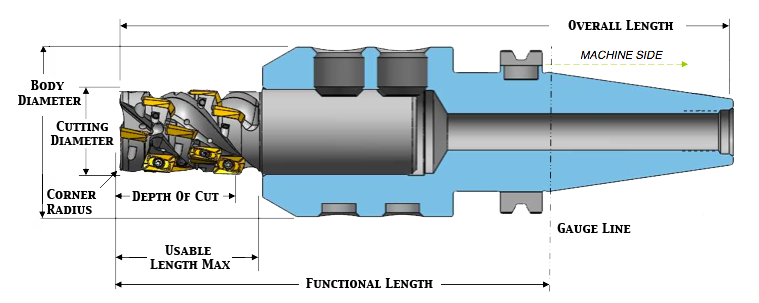
\includegraphics[width=1.0\textwidth]{figures/cutting-tool-measurements.png}
  }
  \caption{Cutting Tool Measurements}
  \label{fig:cutting-tool-measurements}
\end{figure}

\FloatBarrier

The MTConnect Standard will not define the entire geometry of the Cutting Tool, but will provide the information necessary to use the tool in the manufacturing process.  Additional information can be added to the definition of the Cutting Tool by means of schema extensions.

Additional diagrams will reference these dimensions by their codes that will be defined in the measurement tables.  The codes are consistent with the codes used in ISO 13399 and have been standardized.  MTConnect Standard will use the full text name for clarity in the XML document. 

\begin{figure}[ht]
  \centering
  \scalebox{0.7}{
  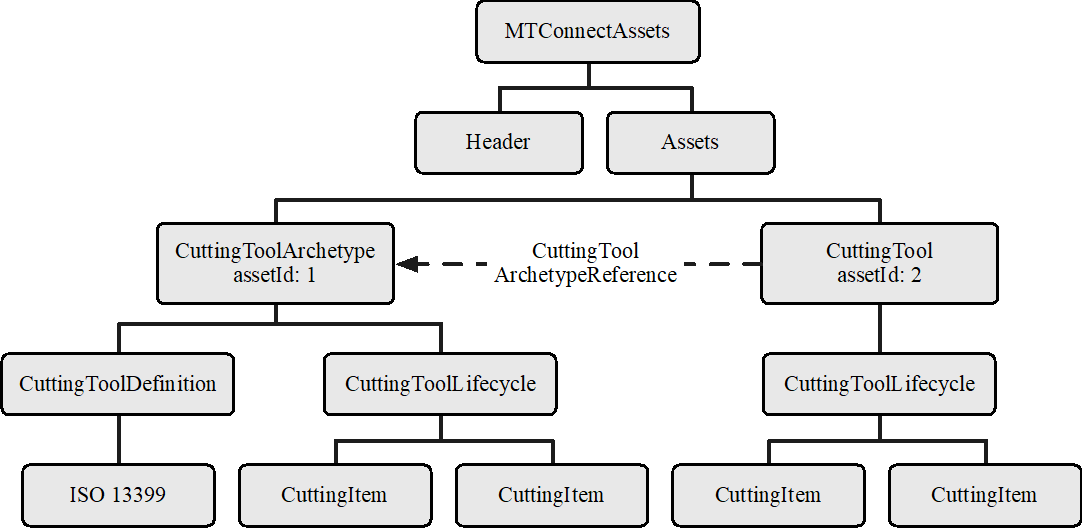
\includegraphics[width=1.0\textwidth]{figures/cutting-tool-asset-structure.png}
  }
  \caption{Cutting Tool Asset Structure}
  \label{fig:cutting-tool-asset-structure}
\end{figure}

\FloatBarrier

The structure of the \gls{mtconnectassets} header is defined in \citetitle{MTCPart1} of the Standard.  A finite number of \glspl{mtconnect asset} will be stored in the \gls{agent}.  This finite number is implementation specific and will depend on memory and storage constraints. The standard will not prescribe the number or capacity requirements for an implementation.

\subsection{Attributes for CuttingToolArchetype}

Refer to \sect{Common Attributes for CuttingTool and CuttingToolArchetype} for a full description of the attributes for \gls{cuttingtoolarchetype} \gls{information model}.

\subsection{Elements for CuttingToolArchetype}

The elements associated with \gls{cuttingtoolarchetype} are given in \tbl{elements-for-cuttingtoolarchetype}.  Each element will be described in more detail below and any possible values will be presented with full definitions.  The elements \MUST be provided in the following order as prescribed by XML.  At least one of \gls{cuttingtooldefinition} or \gls{cuttingtoollifecycle} \MUST be supplied.


\tabulinesep = 5pt
\begin{longtabu} to \textwidth {
    |l|X[2l]|X[0.75l]|}
\caption{Elements for CuttingToolArchetype} \label{table:elements-for-cuttingtoolarchetype} \\

\hline
Element & Description & Occurrence \\
\hline
\endfirsthead

\hline
\multicolumn{3}{|c|}{Continuation of Table \ref{table:elements-for-cuttingtoolarchetype}}\\
\hline
Element & Description & Occurrence \\
\hline
\endhead

\gls{description}	
&
An element that can contain any descriptive content. This can contain configuration information and manufacturer specific details. This element is defined to contain mixed content and XML elements can be added to extend the descriptive semantics of MTConnect Standard.
&
0..1 \\
\hline

\gls{cuttingtooldefinition}	
&
\glsentrydesc{cuttingtooldefinition}
&
0..1 \\
\hline

\gls{cuttingtoollifecycle}	
&
\glsentrydesc{cuttingtoollifecycle}
 The archetype will only contain nominal values.
&
0..1 \\
\hline


\end{longtabu}



\pagebreak

\subsubsection{CuttingToolDefinition Element for CuttingToolArchetype}

\begin{figure}[ht]
  \centering
  \scalebox{0.7}{
  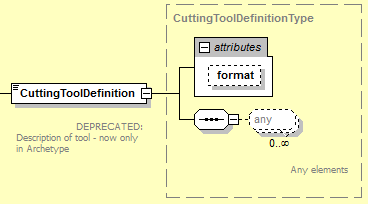
\includegraphics[width=1.0\textwidth]{figures/cuttingtooldefinition-schema.png}
  }
  \caption{CuttingToolDefinition Schema}
  \label{fig:cuttingtool-definition-schema}
\end{figure}

\FloatBarrier

The \gls{cuttingtooldefinition} contains the detailed structure of the Cutting Tool.  The information contained in this element will be static during its lifecycle.  Currently we are referring to the external ISO 13399 standard to provide the complete definition and composition of the Cutting Tool as defined in \sect{CuttingToolLifeCycle}. 

\paragraph{Attributes for CuttingToolDefinition}\mbox{}

\tabulinesep = 5pt
\begin{longtabu} to \textwidth {
    |l|X[3l]|X[0.75l]|}
\caption{Attributes for CuttingToolDefinition} \label{table:attributes-for-cuttingtooldefinition} \\

\hline
Attribute & Description & Occurrence \\
\hline
\endfirsthead

\hline
\multicolumn{3}{|c|}{Continuation of Table \ref{table:attributes-for-cuttingtooldefinition}}\\
\hline
Attribute & Description & Occurrence \\
\hline
\endhead

\gls{format cuttingtooldefinition}
&
\glsentrydesc{format cuttingtooldefinition}
\newline \gls{format cuttingtooldefinition} is an optional attribute.
\newline Valid values of \gls{format cuttingtooldefinition} are – \gls{xml format}, \gls{express format}, \gls{text format}, or \gls{undefined format}.
\newline If \gls{format cuttingtooldefinition} is not specified, the assumed format is \gls{xml format}.
&
0..1 \\
\hline
 

\end{longtabu}

\subparagraph{format Attribute for CuttingToolDefnition}\mbox{}

The \gls{format cuttingtooldefinition} attribute describes the expected representation of the enclosed data. If no value is given, the assumed format will be \gls{xml format}. 

\clearpage

\tabulinesep = 5pt
\begin{longtabu} to \textwidth {
    |l|X[0.75l]|}
\caption{Values for format attribute of CuttingToolDefinition} \label{table:values-for-format-cuttingtooldefinition} \\

\hline
Value & Description\\
\hline
\endfirsthead

\hline
\multicolumn{2}{|c|}{Continuation of Table \ref{table:values-for-format-cuttingtooldefinition}}\\
\hline
Value & Description\\
\hline
\endhead

\gls{xml format}
&
\glsentrydesc{xml format}
\\
\hline

\gls{express format}
&
\glsentrydesc{express format}
\\
\hline

\gls{text format}
&
\glsentrydesc{text format}
\\
\hline

\gls{undefined format}
&
\glsentrydesc{undefined format}
\\
\hline
 

\end{longtabu}

\paragraph{Elements for CuttingToolDefinition}\mbox{}

The only acceptable Cutting Tool definition at present is defined by the ISO 13399 standard.  Additional formats \MAY be considered in the future.

\paragraph{ISO13399 Standard}\mbox{}

The ISO 13399 data \MUST be presented in either XML (ISO 10303-28) or EXPRESS format (ISO 10303-21).  An XML schema will be preferred as this will allow for easier integration with the MTConnect Standard XML tools.  EXPRESS will also be supported, but software tools will need to be provided or made available for handling this data representation.

There will be the root element of the ISO13399 document when XML is used.  When EXPRESS is used the XML element will be replaced by the text representation.


\subsubsection{CuttingToolLifeCycle Element for CuttingToolArchetype}
Refer to \sect{Common Entity CuttingToolLifeCycle} for a complete description of \gls{cuttingtoollifecycle} element.
